Após implementados todos os métodos, foram testados para realizar a minimização quadrática segundo o enunciado:\\

\fbox{\begin{minipage}{34em}
	
	\textbf{2.)} A resposta ao impulso unitário de um sistema foi medida em laboratório,resultando na tabela abaixo\vspace{10pt}
	
	\begin{tabular}{|c||c|c|c|c|c|c|c|c|c|c|}
		\hline
		t$\rightarrow$ & 0.50 & 1.00&1.50 &2.00 &2.50 &3.00 &3.50 &4.00 &4.50 &5.00\\
		\hline
		m(t)$\rightarrow$ & 1.65 & -1.30 &0.50 &-0.10 &-0.15 &0.15 &-0.05 &0.05 &0.01 &0.00\\
		\hline
	\end{tabular}\vspace{10pt}
	
	Deseja-se atribuir a este sistema um modelo LIT caracterizado por \linebreak$H(s)=\omega_n^2/(s^2+2\zeta\omega_ns+\omega_n^2)$ cuja resposta ao impulso unitário é $h(t)=(\omega_n^2/\omega_d)e^{-\zeta\omega_nt}sen(\omega_dt)$, onde $\omega_d=\omega_n\sqrt{1-\zeta^2}$. Pelo método dos mínimos quadrados, encontrar a melhor estimativa para $\zeta$ e $\omega_n$, usando (a) 03 das amostras acima,(b) 05 delas, (c) todas. Comente os resultados obtidos.
	
\end{minipage}}

\vspace{20pt}

Fizemos as operações de encontrar a função objetivo usando os dados $t$ e $m(t)$ da tabela e $h(t)$ e o método mostrado na seção \ref{sec:min_quad}, para 3, 5 e 10 amostras.

Cada uma das três funções objetivo foram testadas em todos os métodos de minimização vetorial implementados durante a realização da matéria de Introdução a Otimização, tantos os métodos ``nobres" (Newton e Gradiente por exemplo) quanto nos métodos ``pobres" mostrados neste documento. Infelizmente, todos os métodos ``nobres" possuíram grande dificuldade, obtendo iterações que duravam minutos tornando assim impossível de computar a minimização.

Nos métodos pobres, O algoritmo genético utilizado neste trabalho mostrou-se eficiente para funções bem comportadas (quadráticas por exemplo), mas em funções menos comportadas, como a função objetivo para 3, 5 e 10 amostras, obteve semelhantemente dificuldades na hora de computar a minimização. Por isso tentou-se utilizar somente duas amostras, e mesmo assim as iterações demoravam dezenas de minutos cada, devido a explosão combinatória na hora da "reprodução".\newpage

A seguir vemos os resultados obtidos para o simplex. As figuras \ref{fig:p_iter_3}, \ref{fig:p_iter_5} e \ref{fig:p_iter_10} mostram a convergência do método e as figuras \ref{fig:p_impulse_3}, \ref{fig:p_impulse_5} e \ref{fig:p_impulse_10}, mostram a resposta ao impulso unitário do sistema proposto pela minimização.\vspace{10pt}\\
Para 3 amostras os valores de $\omega_n$ e $\zeta$ encontrados foram  4.8207 e 0.30037\\
Para 5 amostras os valores de $\omega_n$ e $\zeta$ encontrados foram  2.0521 e 0.30193\\
Para 10 amostras os valores de $\omega_n$ e $\zeta$ encontrados foram  4.9804 e 0.26358\\\\
Fim pelo número de Iterações\\
Iterações: 120/200\\
Tempo de simulação: 5.518\\
Coordenadas do mínimo: (4.8207,0.30037,0.0019568)\\\\
Fim pelo tamanho do Raio da Circunferência Circunscrita\\
Iterações: 69/200\\
Tempo de simulação: 3.628\\
Coordenadas do mínimo: (2.0521,0.30193,0.42709)\\\\
Fim pelo tamanho do Raio da Circunferência Circunscrita\\
Iterações: 71/200\\
Tempo de simulação: 3.837\\
Coordenadas do mínimo: (4.9804,0.26358,0.011948)\\





\twocolumn
\begin{figure}[H]
	\begin{center}	
		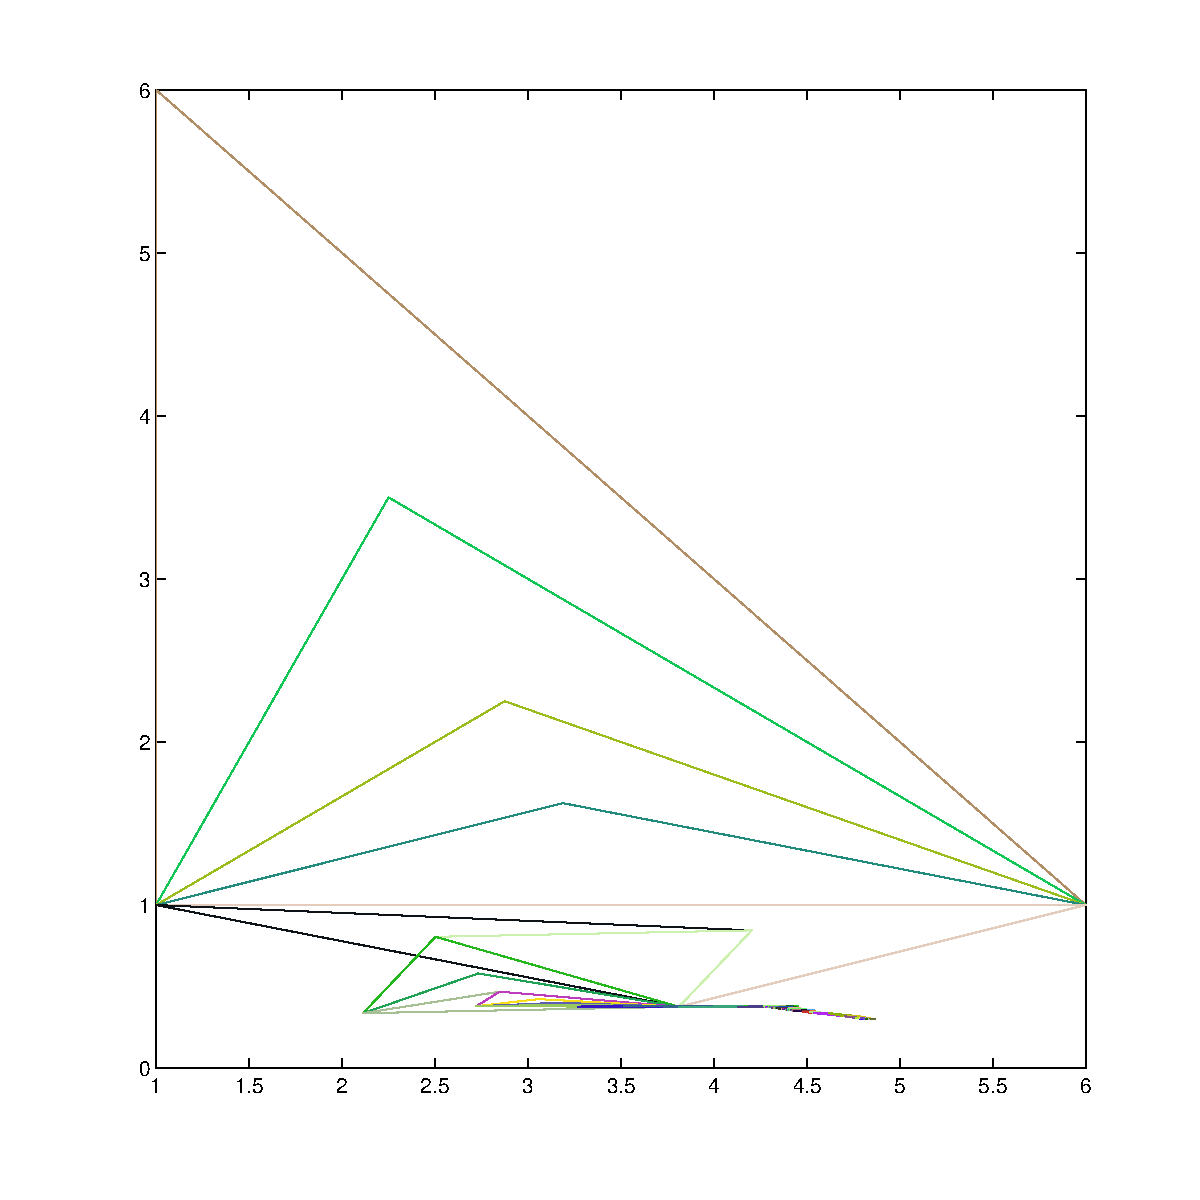
\includegraphics[width=6cm]{Plots/p_iter_3.pdf}
		\caption{Convergência para 3 amostras}
		\label{fig:p_iter_3}
	\end{center}
\end{figure}

\begin{figure}[H]
	\begin{center}	
		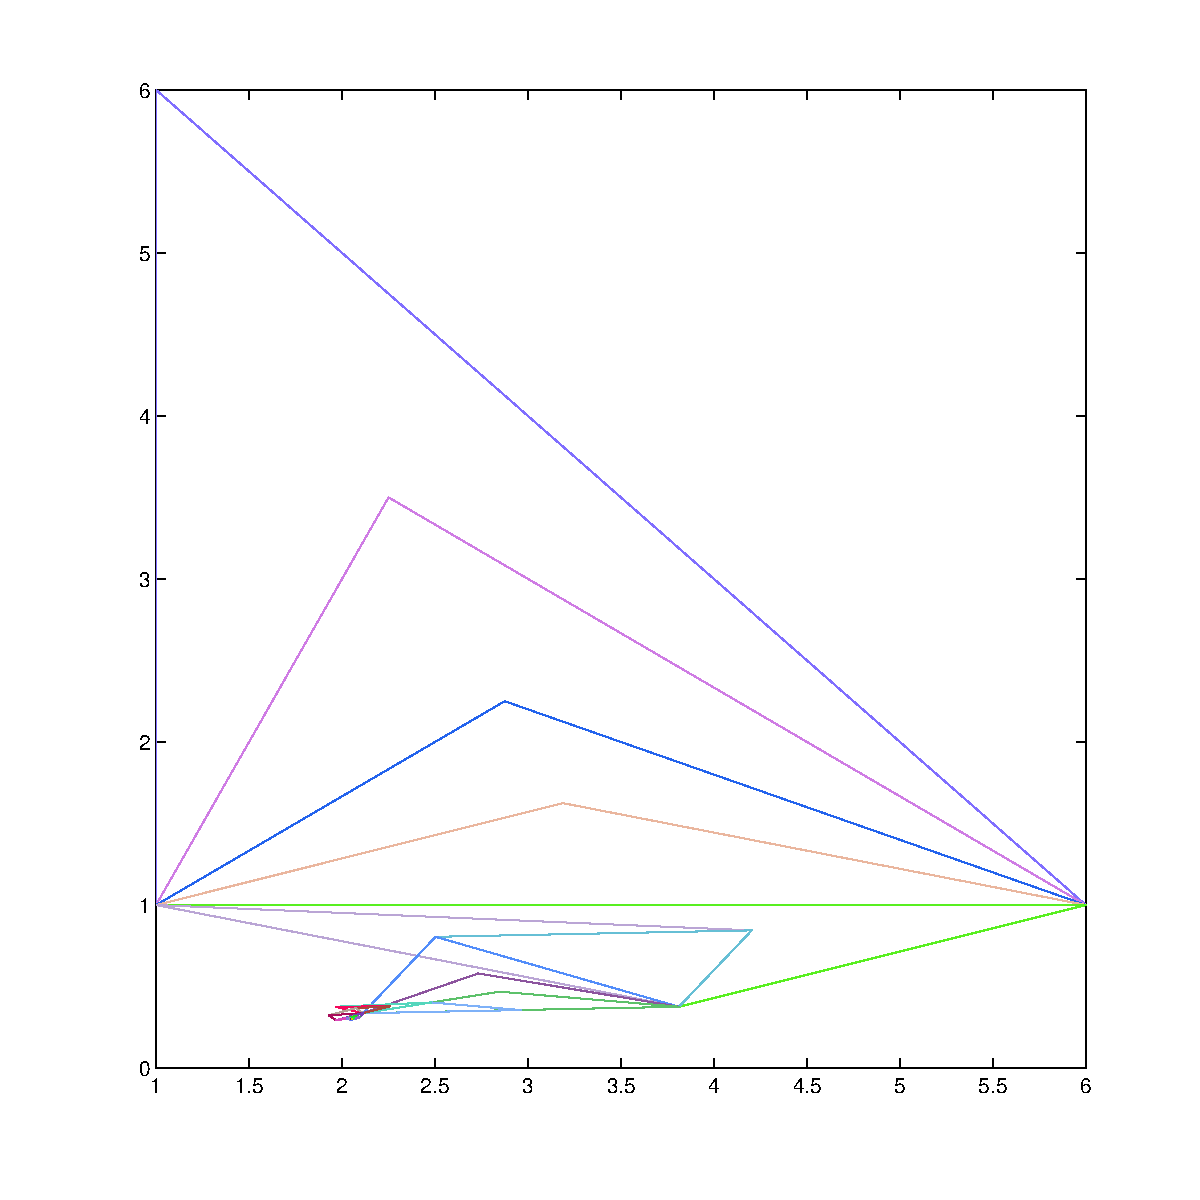
\includegraphics[width=6cm]{Plots/p_iter_5.pdf}
		\caption{Convergência para 5 amostras}
		\label{fig:p_iter_5}
	\end{center}
\end{figure}

\begin{figure}[H]
	\begin{center}	
		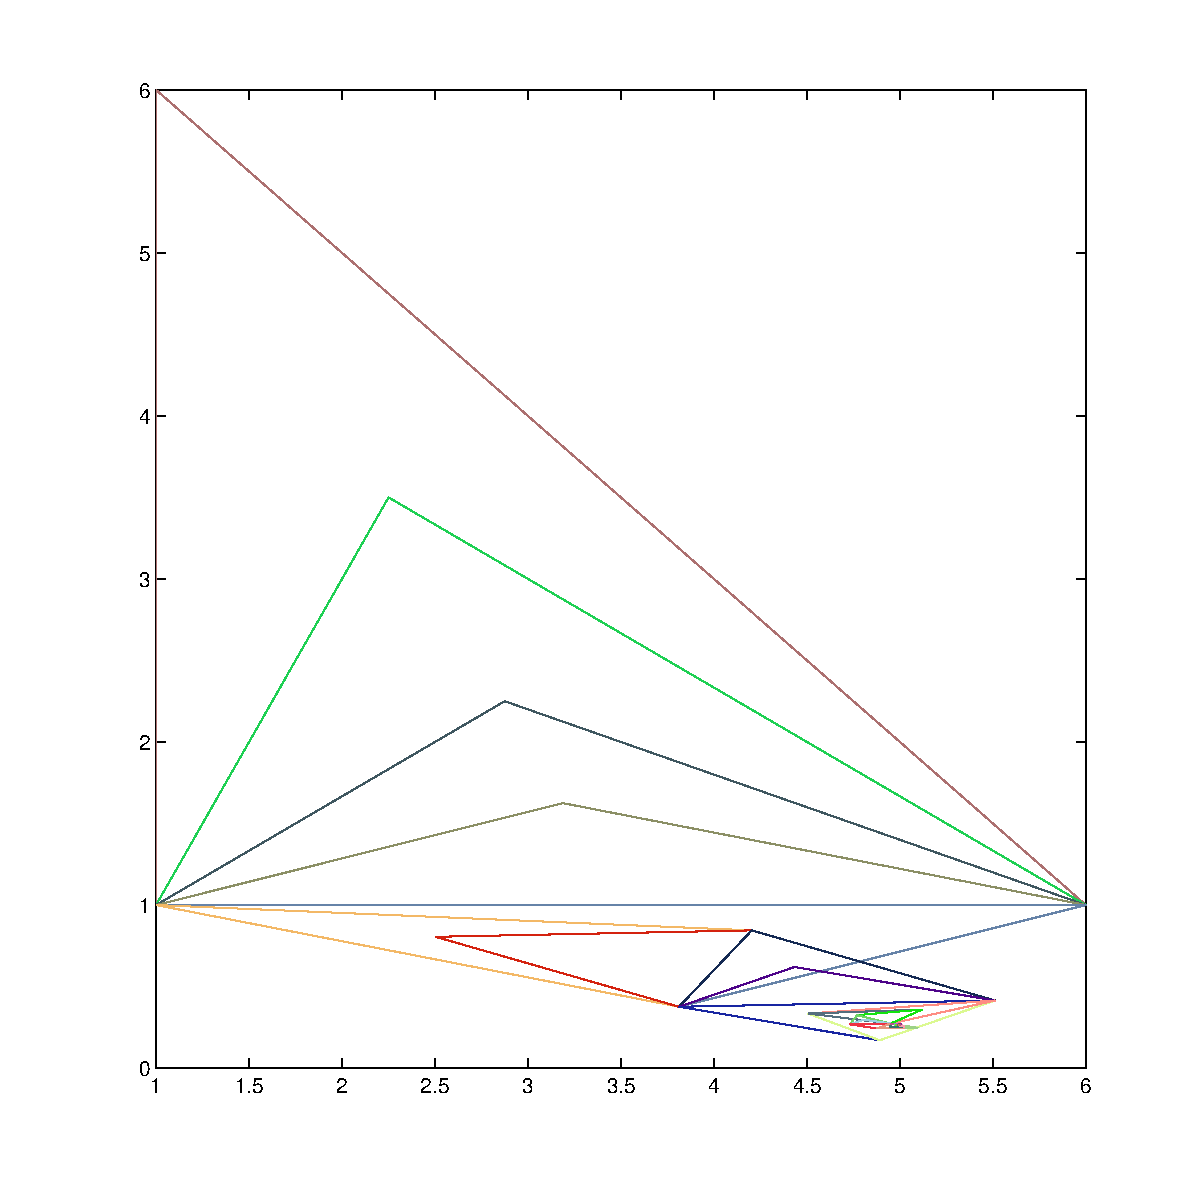
\includegraphics[width=6cm]{Plots/p_iter_10.pdf}
		\caption{Convergência para 10 amostras}
		\label{fig:p_iter_10}
	\end{center}
\end{figure}



\begin{figure}[H]
	\begin{center}	
		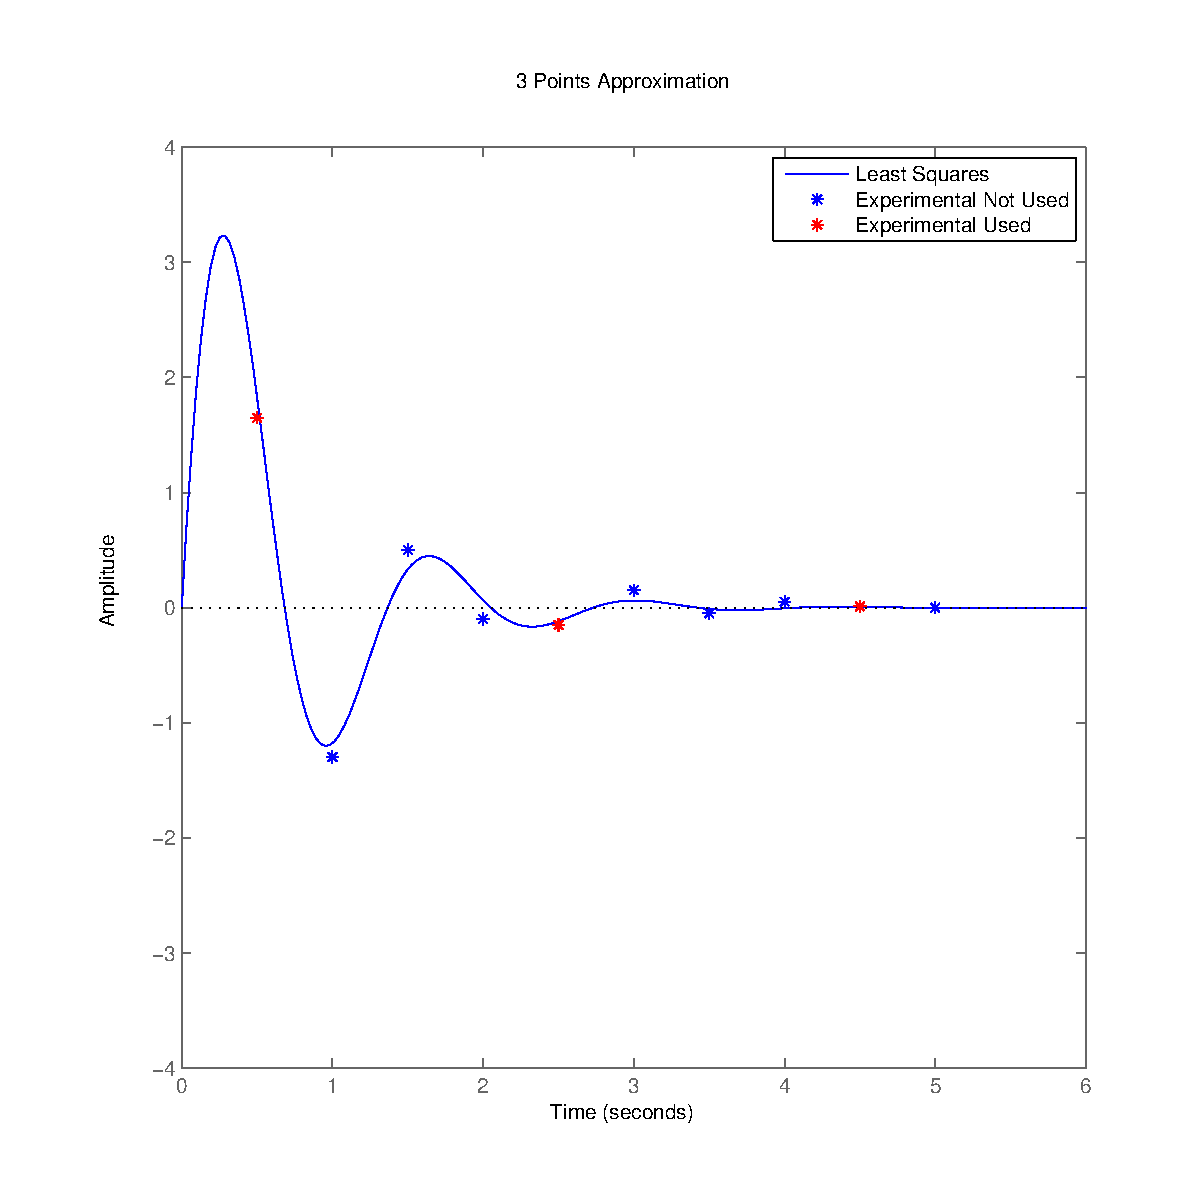
\includegraphics[width=6cm]{Plots/p_impulse_3.pdf}
		\caption{Resposta do impulso (3 amostras)}
		\label{fig:p_impulse_3}
	\end{center}
\end{figure}

\begin{figure}[H]
	\begin{center}	
		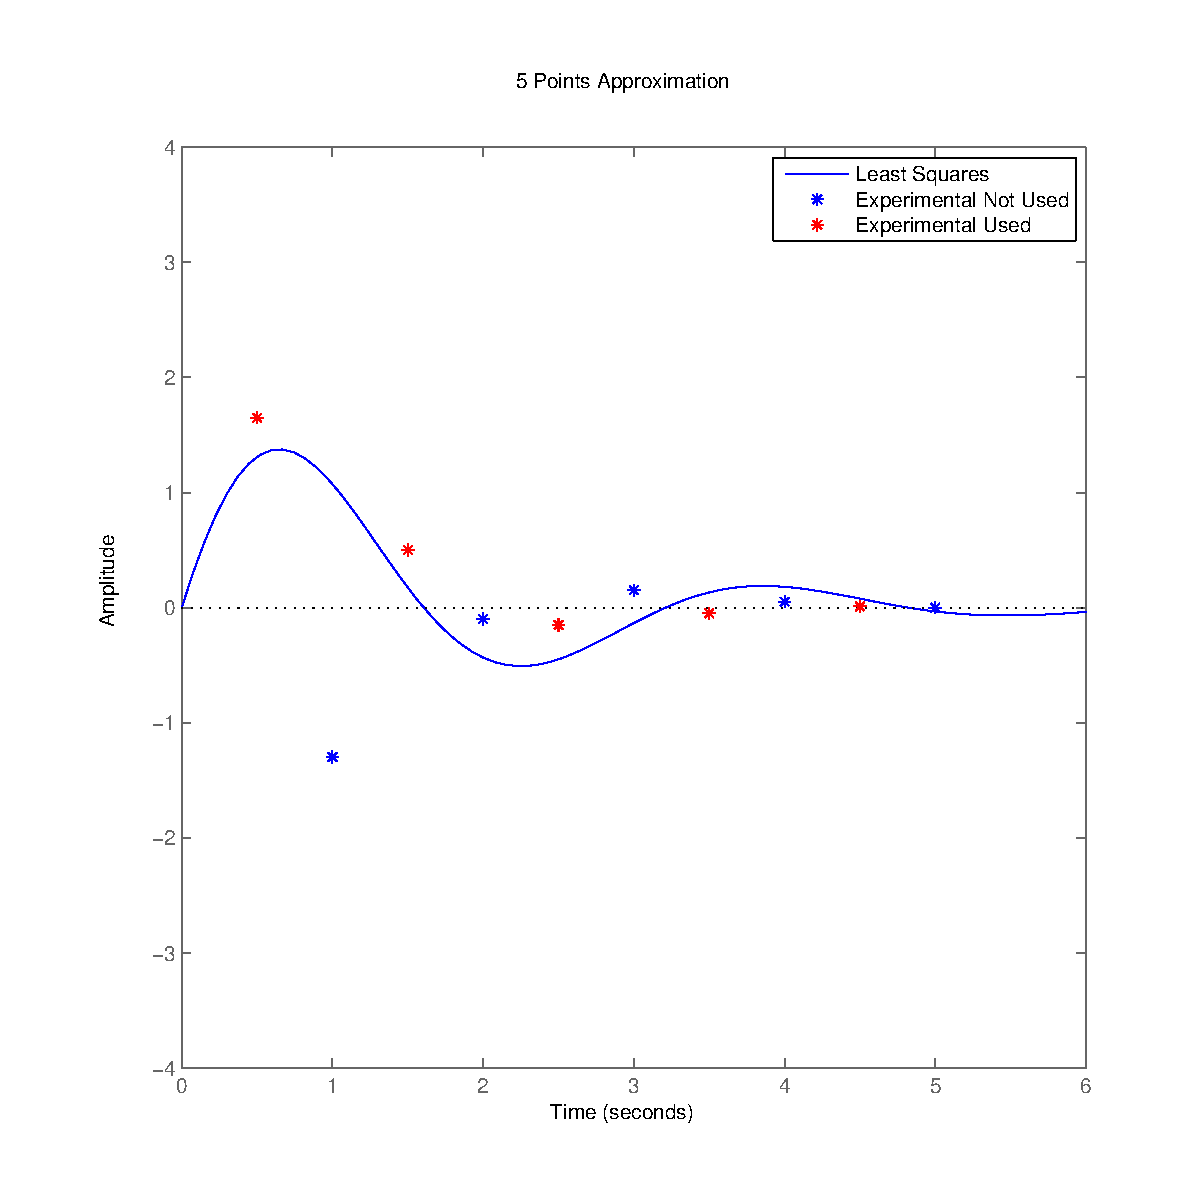
\includegraphics[width=6cm]{Plots/p_impulse_5.pdf}
		\caption{Resposta do impulso (5 amostras)}
		\label{fig:p_impulse_5}
	\end{center}
\end{figure}

\begin{figure}[H]
	\begin{center}	
		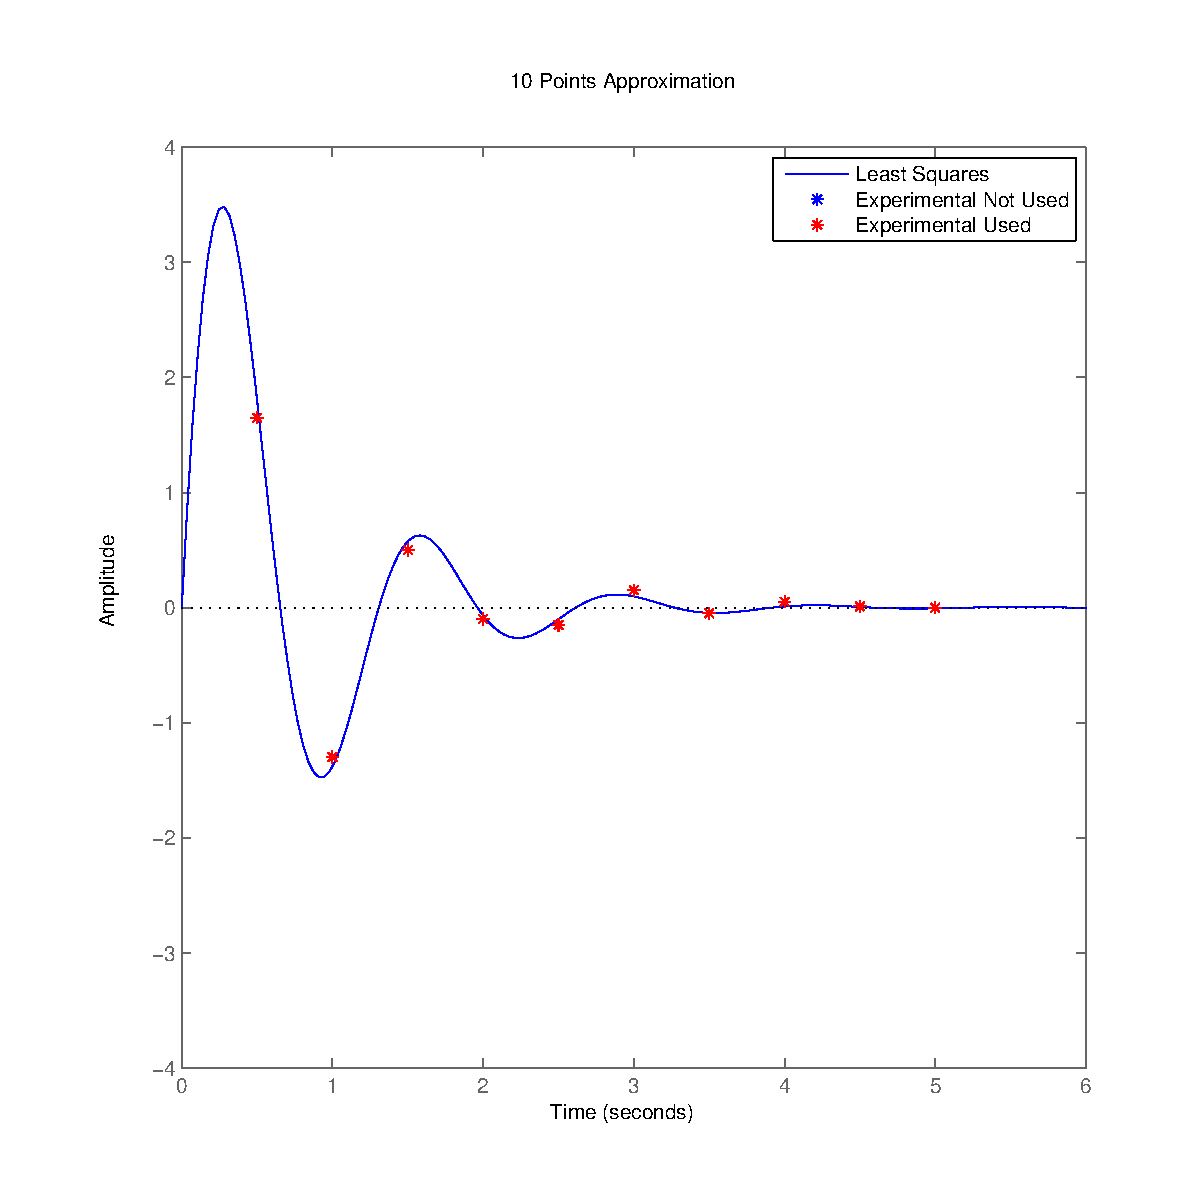
\includegraphics[width=6cm]{Plots/p_impulse_10.pdf}
		\caption{Resposta do impulso (10 amostras)}
		\label{fig:p_impulse_10}
	\end{center}
\end{figure}
\onecolumn
\newpage

